\section{Evaluation}


In this section, we evaluate the proposed optimization, where we analyze our
improvements on code-size reduction, as well as its impact on the program's
performance and compilation-time.

%\begin{figure}[t!]
%  \centering
%  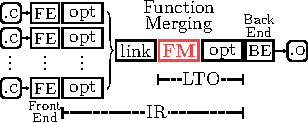
\includegraphics[width=0.7\linewidth]{figs/opt-pipeline.pdf}
%  \caption{The compilation pipeline using a monolithic link-time optimization (LTO).}
%  \label{fig:opt-pipeline}
%\end{figure}



\subsection{Experimental Setup}
We compare our optimization with the state-of-the-art function merging approach~\cite{edler14}, and the LLVM's implementation of identical
function merging. All optimizations are implemented in LLVM v7 and evaluated using the C/C++ SPEC CPU2006~\cite{spec} benchmark suite.

We apply all approaches to an Intel and an ARM platforms. The Intel platform has a quad-core 3.4~GHz Intel Core i7 CPU with 16~GiB of RAM.
%The operating system is openSUSE 42.2 with Linux kernel version 4.4.27.
The ARM platform has a Cortex-A53 ARMv8 CPU of 1.4~GHz with 1~GiB of RAM.
%The operating system of the ARM platform is a Raspbian.
We also use the Intel platform to cross-compile all benchmarks to the ARM
platform.
For this reason, we only show compilation-time results for the Intel platform.

\begin{figure*}[t!]
  \centering
  %\subfigure[Intel platform.]{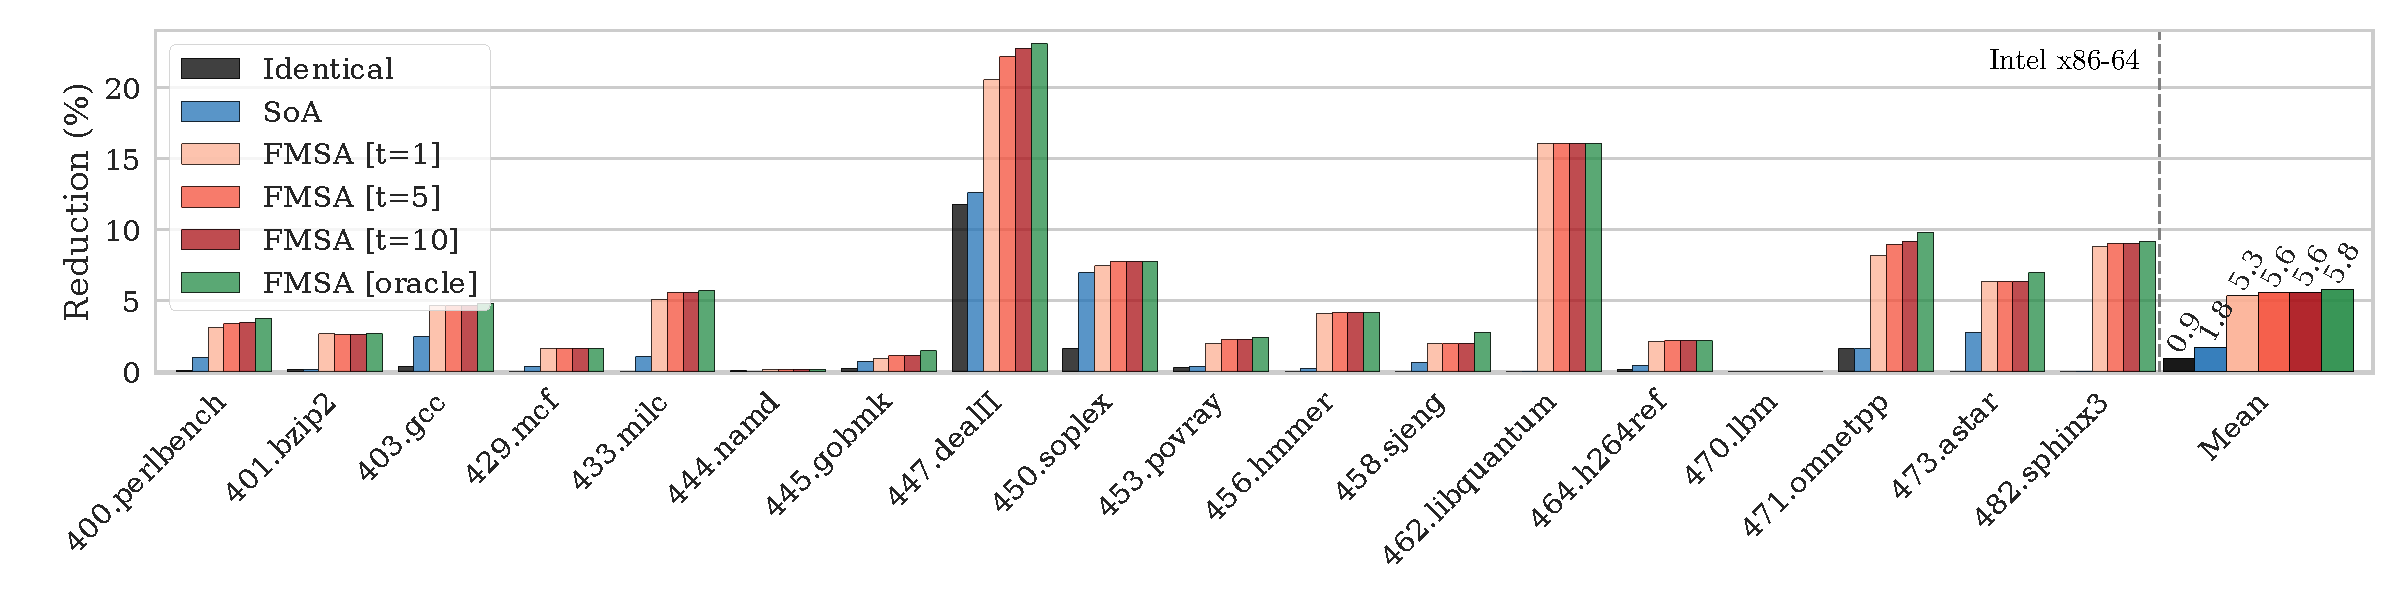
\includegraphics[width=\linewidth]{figs/reduction-obj-intel-label.pdf}}
  %\subfigure[ARM platform.]{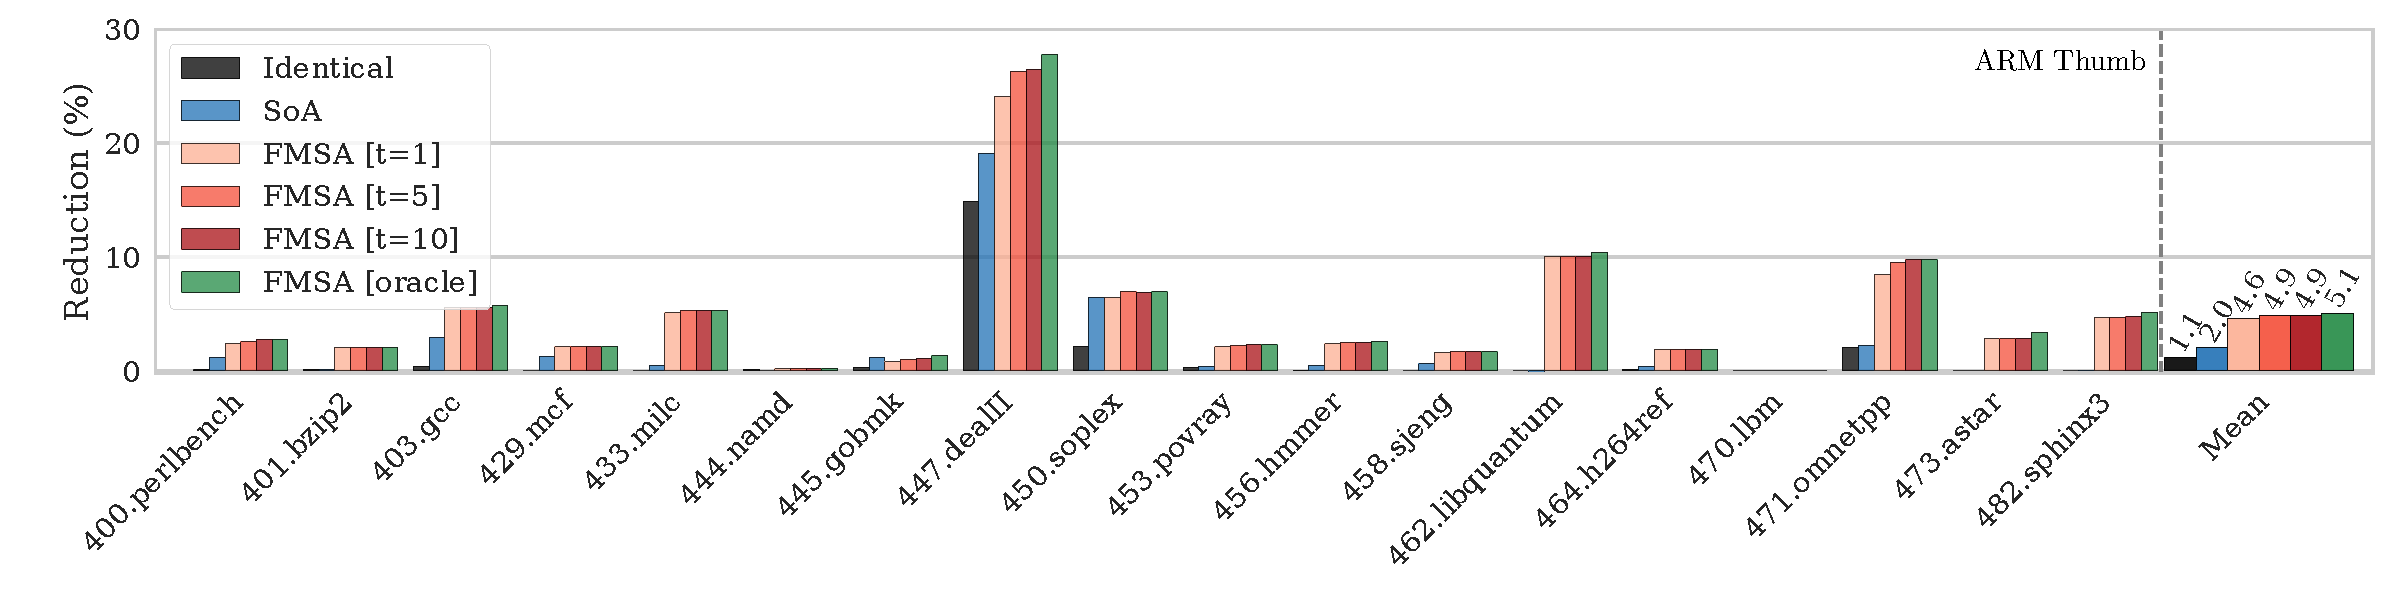
\includegraphics[width=\linewidth]{figs/reduction-obj-arm-label.pdf}}
  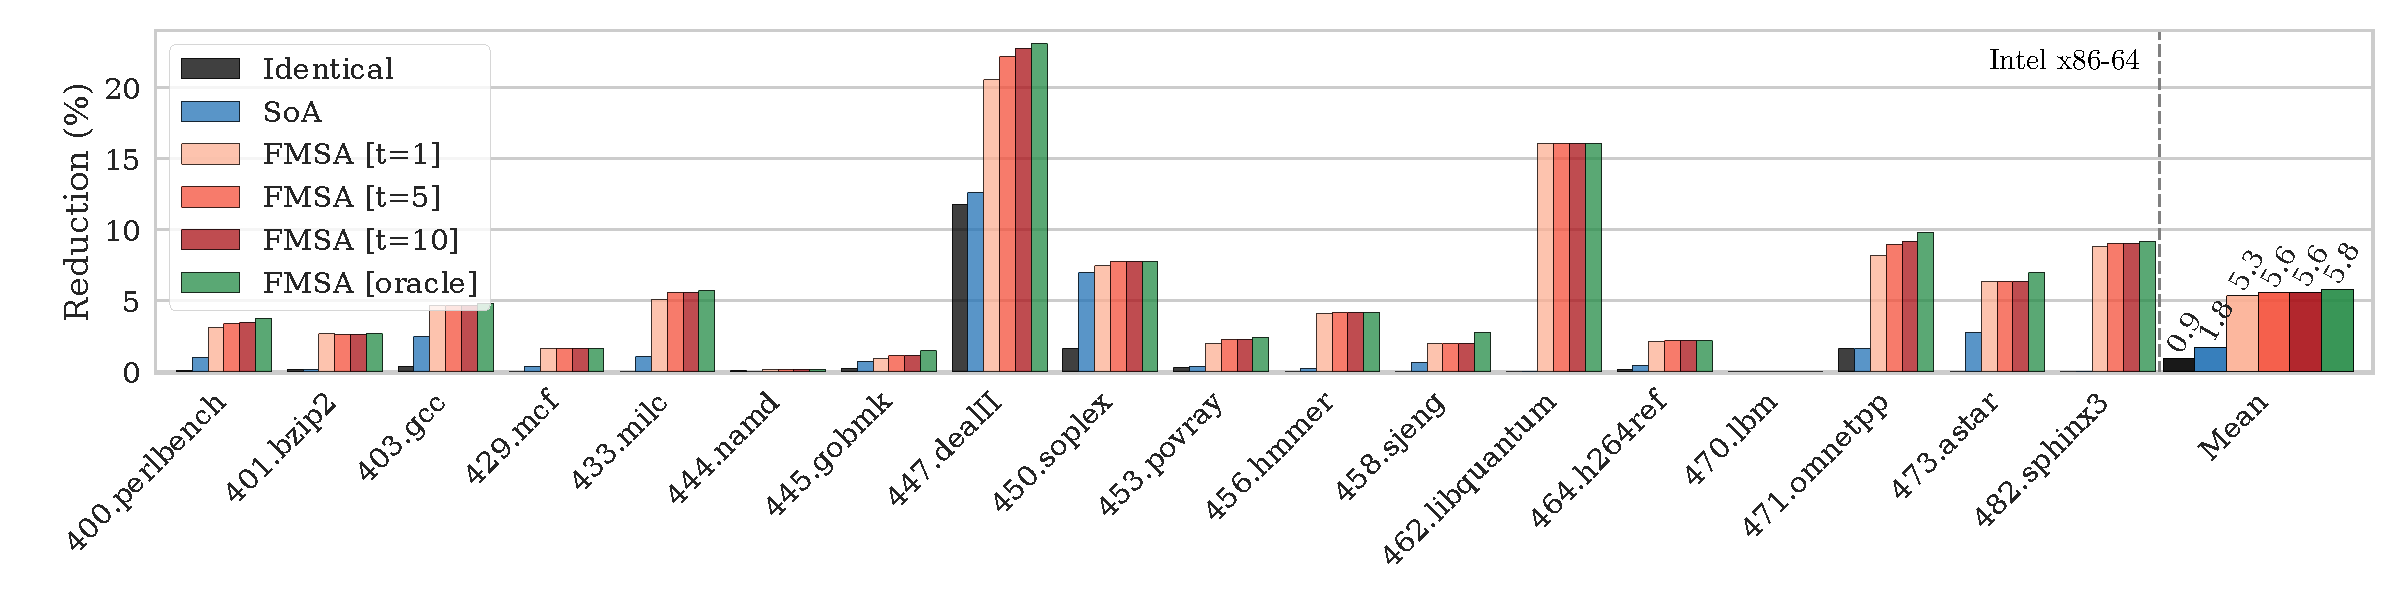
\includegraphics[width=\linewidth]{figs/reduction-obj-intel-label.pdf} \\
  \vspace{-1.8ex}
  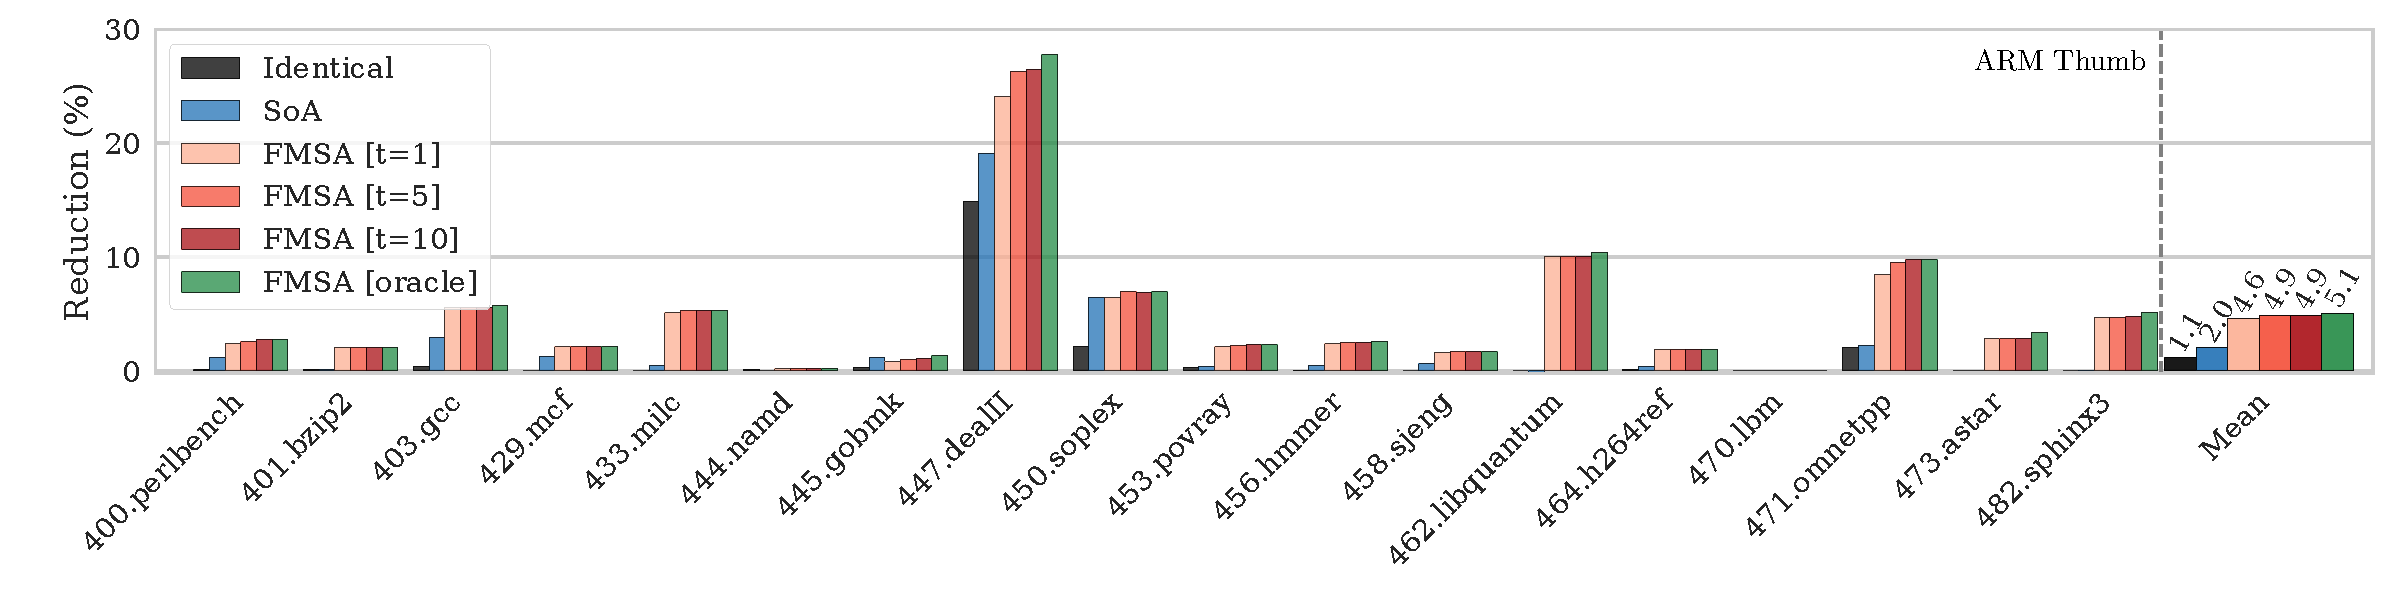
\includegraphics[width=\linewidth]{figs/reduction-obj-arm-label.pdf}
  \vspace{-4ex}
  \caption{Reduction on the object file for both the Intel (top) and ARM (bottom) platforms.}
  \label{fig:reduction-obj}
\end{figure*}


During our evaluation, we refer to LLVM's identical function merging as \textit{Identical}, the state-of-the-art as \textit{SoA}, and our
proposed function merging as \textit{FMSA}. For the proposed optimization, we vary the exploration threshold (Section~\ref{sec:framework})
and we present the results for a range of those values. In addition, we also show the results for the oracle exploration strategy, which
instead of using a rank-based greedy approach, actually executes the merge operation with all candidates and then chooses the best one.
%The oracle represents the results assuming a perfect ranking strategy.
%However, the oracle has a very costly quadratic exploration, as explained in
%Section~\ref{sec:framework}.
The oracle represents the results assuming a perfect ranking strategy, which requires a very costly quadratic exploration, as explained in
Section~\ref{sec:framework}. \fixme{ZW: I suggest we call ``oracle" exhaustive-exploration instead. ``oracle" often used to refer the
up-bound performance.}



\subsection{Code-Size Reduction}

\begin{figure*}[t]
  \centering
  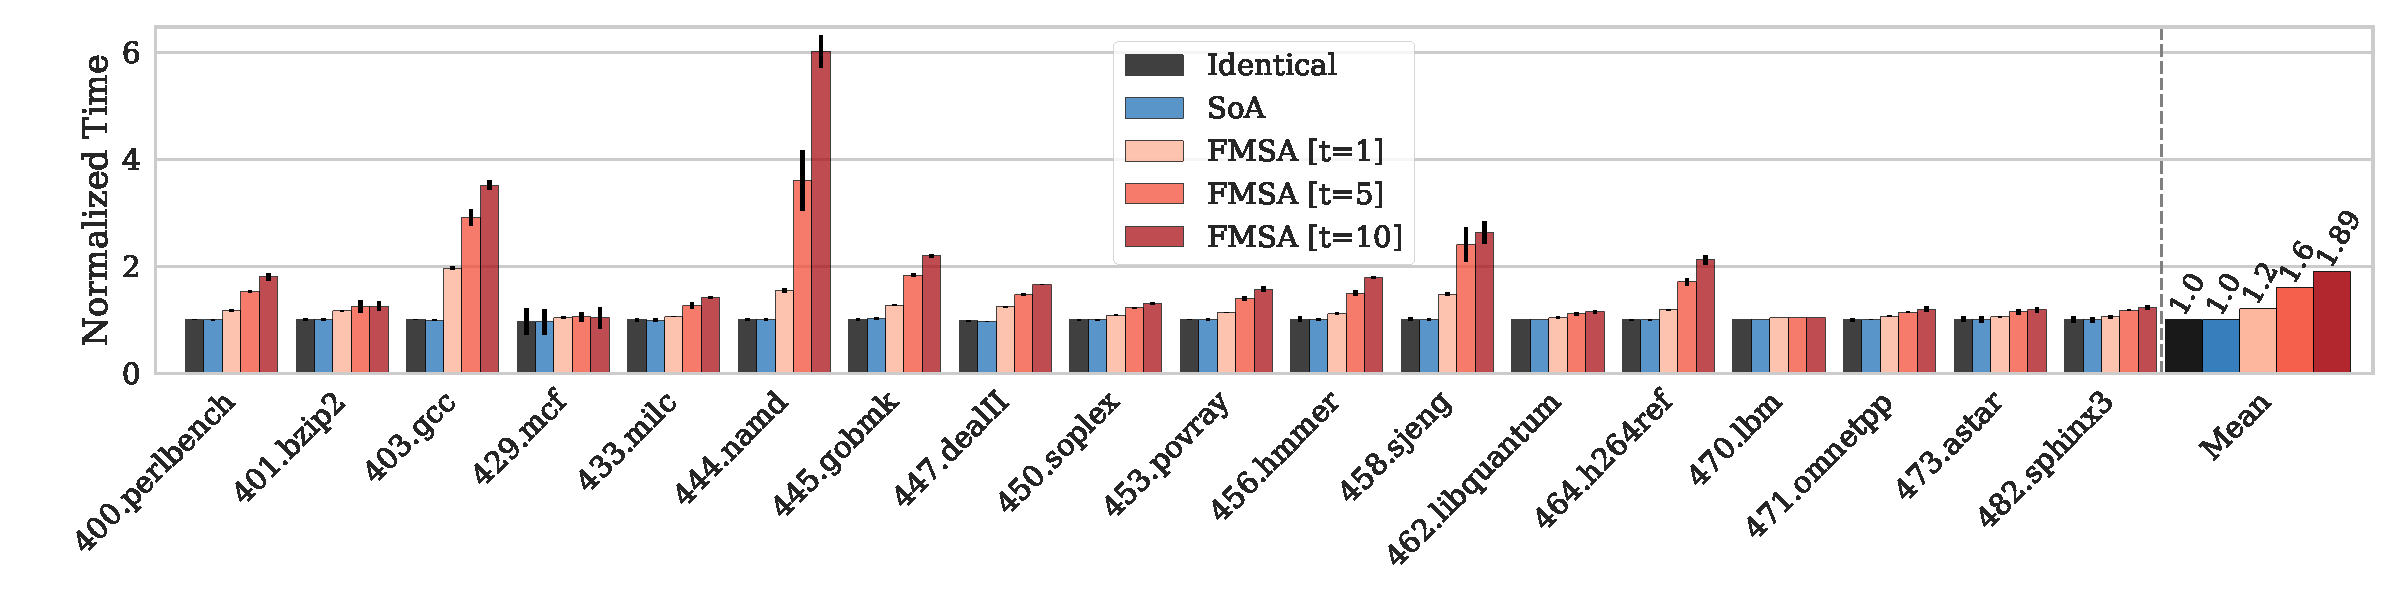
\includegraphics[width=\linewidth]{figs/compilation-time.pdf}
  \vspace{-4ex}
  \caption{Compilation-time overhead on the Intel platform. The oracle has an average overhead of 25$\times$.}
  \label{fig:compilation-time}
\end{figure*}

%\begin{figure*}[th]
%  \centering
%  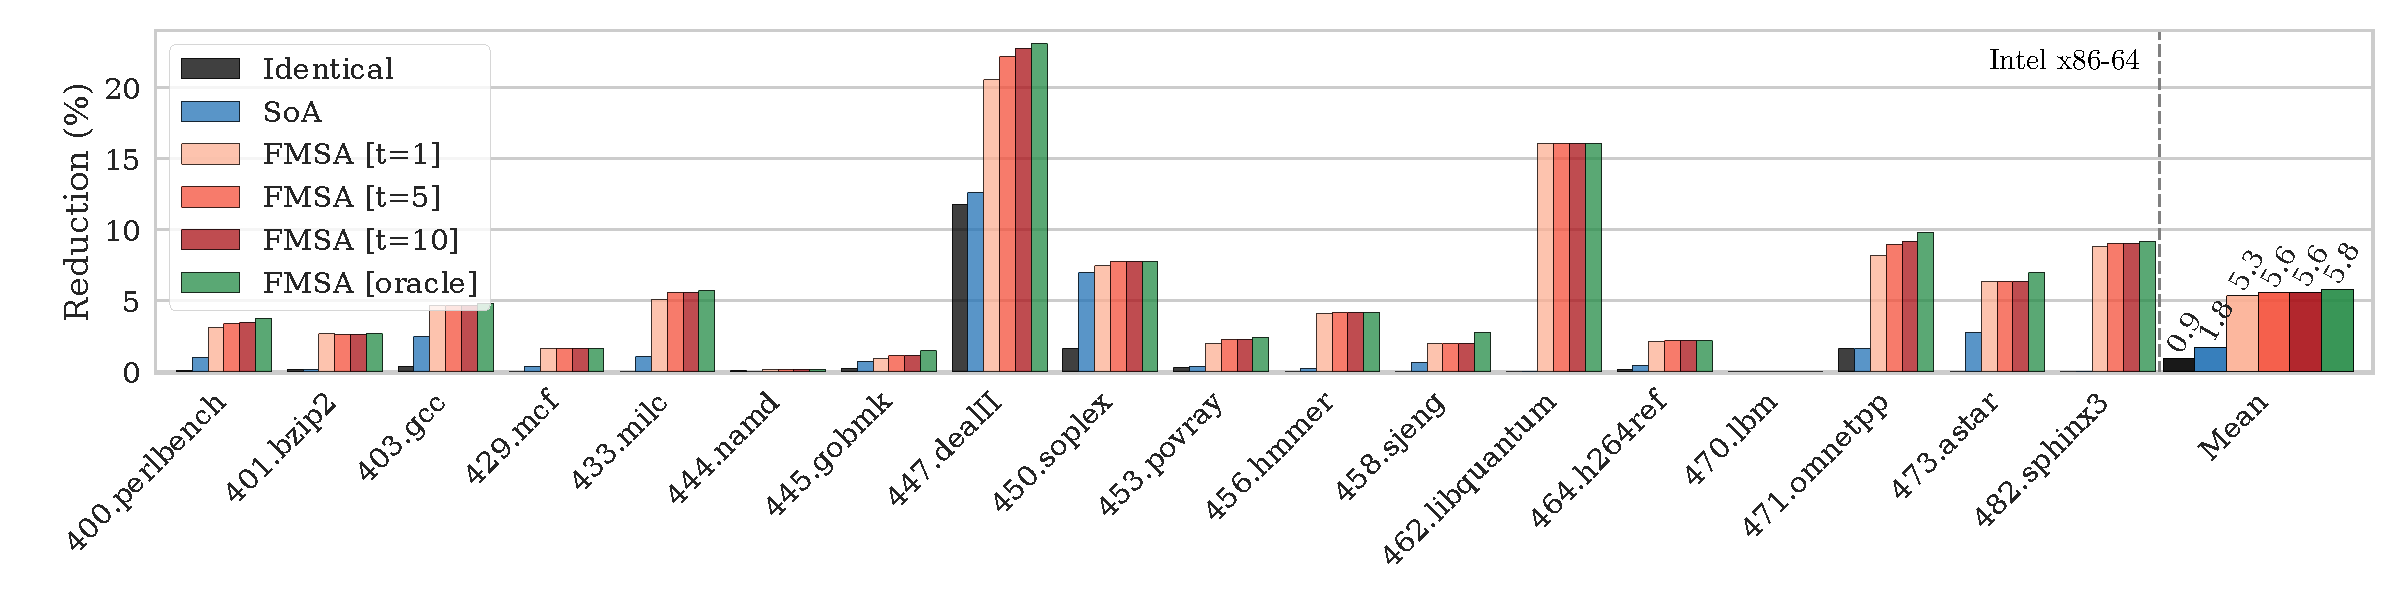
\includegraphics[width=\linewidth]{figs/reduction-obj-intel-label.pdf}
%  \caption{Reduction on the object file for the Intel architecture.}
%  \label{fig:reduction-obj-intel}
%\end{figure*}
%\begin{figure*}[th]
%  \centering
%  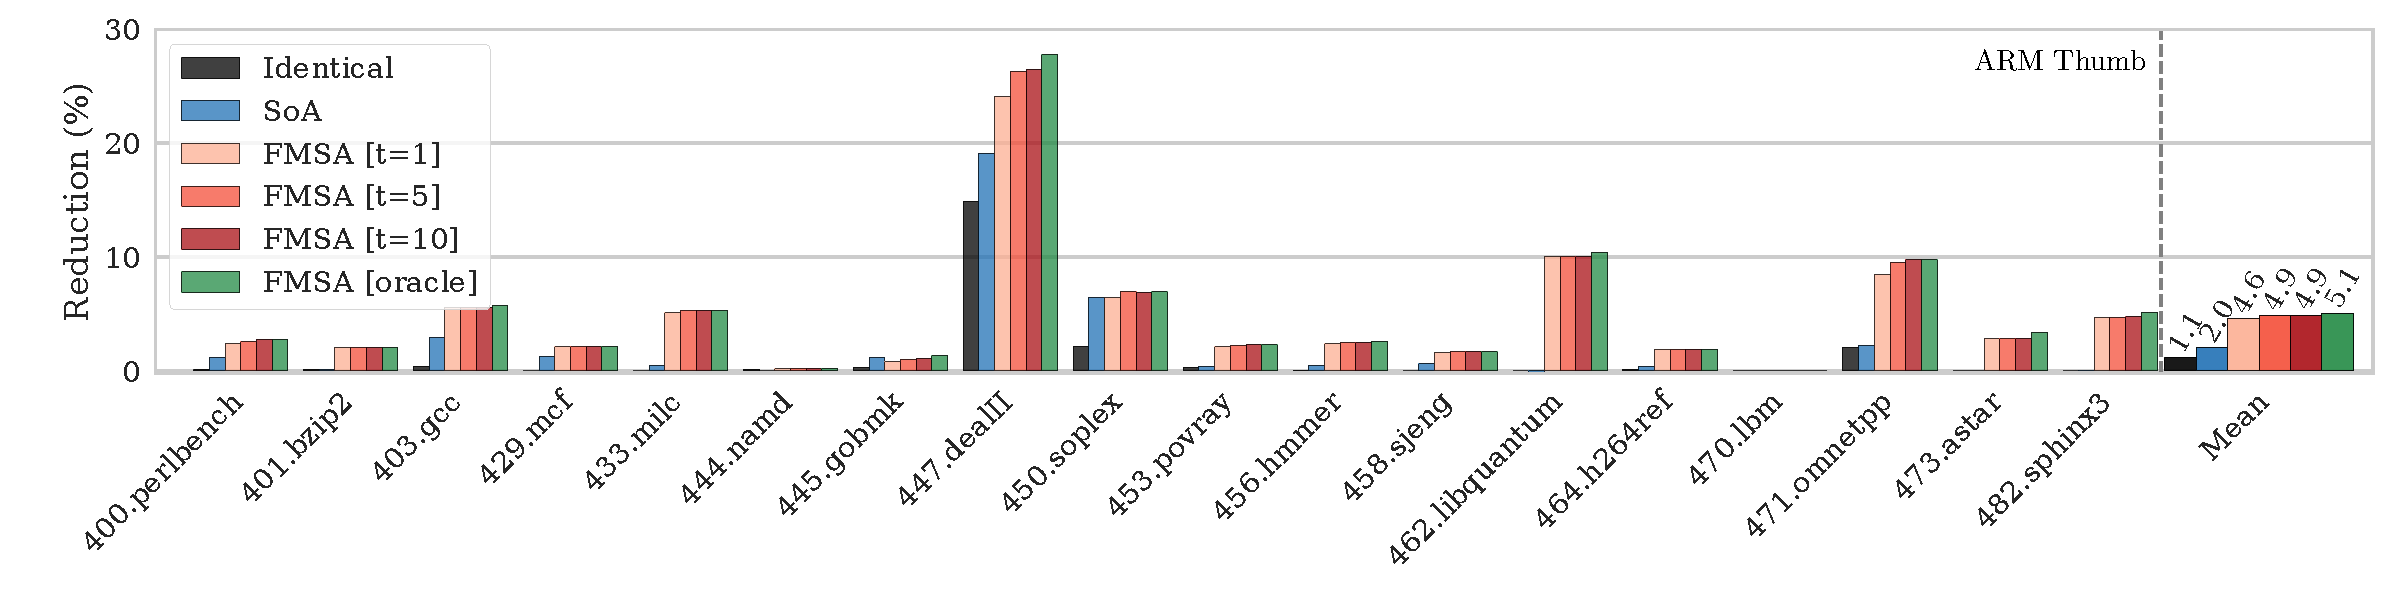
\includegraphics[width=\linewidth]{figs/reduction-obj-arm-label.pdf}
%  \caption{Reduction on the object file for the ARM architecture.}
%  \label{fig:reduction-obj-arm}
%\end{figure*}


Figure~\ref{fig:reduction-obj} reports the code-size reduction over the baseline for the linked object. %These results show how much we can improve over the existing techniques, by having a more powerful solution, and how close we
%can get to the oracle with our ranking-based exploration framework.
We observe a similar pattern for code-size reduction for all benchmarks on the Intel and ARM architectures. This is expected because the
optimizations are applied at the platform-independent IR level. However, some of the decisions may change due to the target-dependent cost
model (LLVM's TTI) and, similarly, the final object files will also differ due to differences in the instruction set architecture (ISA),
compiler backend, etc.

Our approach, FMSA, significantly improves over the state-of-the art (SoA). For the Intel platform, FMSA can achieve an average code-size
reduction of up to 5.8\% (or 5.3\% with the lower configuration), while the SoA and Identical had an average reduction of 1.8\% and 0.9\%,
respectively. Similarly, for the ARM platform, FMSA can achieve an average code-size reduction of up to 5.1\% (or 4.6\% with the lower
configuration), while the SoA and Identical had an average reduction of 2\% and 1.1\%, respectively. For several of the benchmarks, the
proposed technique shows some impressive code-size reductions compared to the other optimizations. Table~\ref{tab:reduction} highlights
some of these results for both platforms. Although not noticeable in Figure~\ref{fig:reduction-obj}, the state-of-the-art slightly
increases code-size in two benchmarks, namely, \texttt{462.libquantum} and \texttt{482.sphinx3}, while FMSA shows significant reductions in
both cases. The only case where a configuration of FMSA results in slightly less code-size saving over the SoA is on the \texttt{445.gobmk}
benchmark on the ARM platform. However, the oracle is able to improve over the SoA, with a code-size reduction of 1.33\%. In all other
cases, FMSA is always equal or better than all other function-merging optimizations, usually by a significant margin.

\begin{table}[]
\label{tab:reduction}
\centering
\scalebox{0.8}{
\begin{tabular}{lccc}
\toprule
\multicolumn{1}{c}{\textbf{Benchmarks}} & \textbf{Identical} & \textbf{SoA}  & \textbf{FMSA {[}t=1{]}} \\
\midrule
%%%400.perlbench                             & 0.09 / 0.09        & 1.03 / 1.15   & 3.13 / 2.40             \\ \hline
\rowcolor{evencolor} 401.bzip2                                 & 0.15 / 0.16        & 0.15 / 0.16   & 2.67 / 2.09             \\
%%%403.gcc                                   & 0.36 / 0.43        & 2.48 / 2.89   & 4.71 / 5.59             \\ \hline
%%%429.mcf                                   & 0 / 0              & 0.41 / 1.29    & 1.66 / 2.11             \\ \hline
433.milc                                  & 0 / 0              & 1.08 / 0.46   & 5.09 / 5.12             \\
%%%444.namd                                  & 0.10 / 0.14        & 0 / 0         & 0.20 / 0.17             \\ \hline
\rowcolor{evencolor} 447.dealII                                & 11.77 / 14.83      & 12.59 / 19.12 & 20.57 / 24.08           \\
445.gobmk                                 & 0.26 / 0.32        & 0.77 / 1.15   & 0.96 / 0.78             \\
%%%450.soplex                                & 1.62 / 2.16        & 6.99 / 6.47   & 7.46 / 6.48             \\ \hline
\rowcolor{evencolor} 453.povray                                & 0.28 / 0.33        & 0.38 / 0.40   & 2.04 / 2.12             \\
456.hmmer                                 & 0 / 0              & 0.27 / 0.50   & 4.15 / 2.40             \\
%%%458.sjeng                                 & 0 / 0              & 0.63 / 0.63   & 1.97 / 1.62             \\ \hline
\rowcolor{evencolor} 462.libquantum                            & 0 / 0              & -0.07 / -0.17 & 16.08 / 10.04           \\
%%%464.h264ref                               & 0.16 / 0.14        & 0.47 / 0.40   & 2.16 / 1.86             \\ \hline
%%%470.lbm                                   & 0 / 0              & 0 / 0         & 0 / 0                   \\ \hline
471.omnetpp                               & 1.65 / 2.08        & 1.64 / 2.27   & 8.18 / 8.47             \\
\rowcolor{evencolor} 473.astar                                 & 0 / 0              & 2.76 / 0      & 6.33 / 2.81             \\
482.sphinx3                               & 0 / 0              & -0.06 / 0.06  & 8.85 / 4.72             \\
\bottomrule
\end{tabular}
}
\caption{Highlights of code reduction results (in percentages) on \textit{Intel / ARM} platforms. }
\end{table}


%These results show that, although it has
%little compilation-time overhead,
%merging identical functions, in most cases, has a rather small impact on
These results show that, although the LLVM's identical function merging has
little compilation-time overhead, in most cases, it also has a rather small
impact on code-size reduction, with an average reduction of less than 1\%.
The only few cases where it has a noticeable impact are on some of the C++
benchmarks, namely, 447.dealII, 450.soplex, and 471.omnetpp, which is mostly
due to the heavy use of templating. %, as exemplified in Figure~\ref{fig:identical-example}.
%However, the proposed technique (FMSA) can also perform much better on these
However, FMSA can also perform much better on these
benchmarks, with an improvement of almost 6$\times$ on the 471.omnetpp benchmark.
Moreover, our technique also shows remarkable reductions on several of the
C benchmarks, such as, 462.libquantum and 482.sphinx3, especially when taking into
account that the other techniques have no real impact on these benchmarks.

%Figure~\ref{fig:libquantum-example} shows an example of two functions\footnote{We
%have changed very lightly some of the names used in the functions so that the
%code fits nicely in the paper. The original names of the functions are:
%quantum\_cond\_phase and quantum\_cond\_phase\_inv.}
%from the 462.libquantum benchmark that are merged by the proposed optimization.
%The proposed function-merging technique is the \textit{first} technique able to
%merge these two functions.
%Although they are very similar functions, the state-of-the-art is unable to
%merge them since their CFGs are not structurally identical.
%For the proposed optimization, however, these two functions receive a similarity
%score above $0.49$, which puts them at the top of the rank, and the
%profitability cost model estimates a code-size reduction of 40\%.
%Overall, our optimization was able to merge nine pairs of functions for the
%462.libquantum benchmark.
%Similar to the example shown, all of them were top ranked based on their
%fingerprint similarity.

%Note that functions that are identical at the IR or machine level are not
%necessarily identical at the source level.
%Figure~\ref{fig:identical-example} shows two real functions extract from the
%447.dealII program in the SPEC CPU2006~\cite{spec} benchmark suite.
%Although these two functions are not identical at the source level, they become
%identical after a template specialization and some optimizations are applied, in
%particular, constant propagation, constant folding, and dead-code elimination.
%Specializing \verb|dim| to $1$ enables to completely remove the loop in the
%function \verb|PolynomialSpace|.
%Similarly, specializing \verb|dim| to $1$ results in only the first iteration
%of the loop in the function \verb|TensorProductPolynomials| being executed.
%The compiler is able to statically analyze and simiplify the loops in both
%functions, resulting in the identical functions shown at the bottom of
%Figure~\ref{fig:identical-example}.


%\begin{figure*}[t]
%  \centering
%  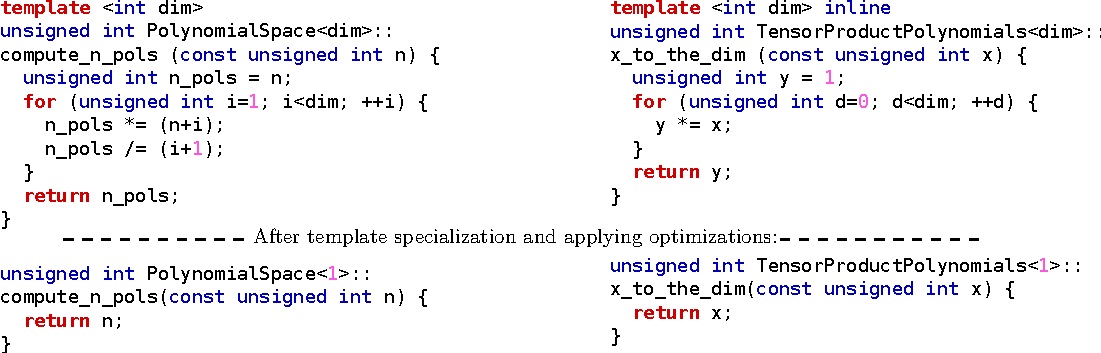
\includegraphics[width=0.95\linewidth]{figs/identical-example.pdf}
%  \caption{Two function extracted from the 447.dealII benchmark that are not
%           identical at the source level, but after applying template
%           specialization and optimizations they become identical at the IR
%           level.}
%  \label{fig:identical-example}
%\end{figure*}


\subsection{Compilation Overhead}


Figure~\ref{fig:compilation-time} shows the compilation-time overhead for all
optimizations.
We are only showing results for the Intel machine, since the benchmarks were
also cross-compiled from this Intel machine to the ARM platform.
We are not presenting the results for the oracle exploration because its very
large overhead would make it impossible to visualize the results properly.
The oracle has an average compilation-time overhead of 25$\times$ compared to
the baseline, with its largest overhead being of 136$\times$ on the 447.dealII
benchmark.

\begin{figure}[b]
  \centering
  %\hspace{-2ex}
  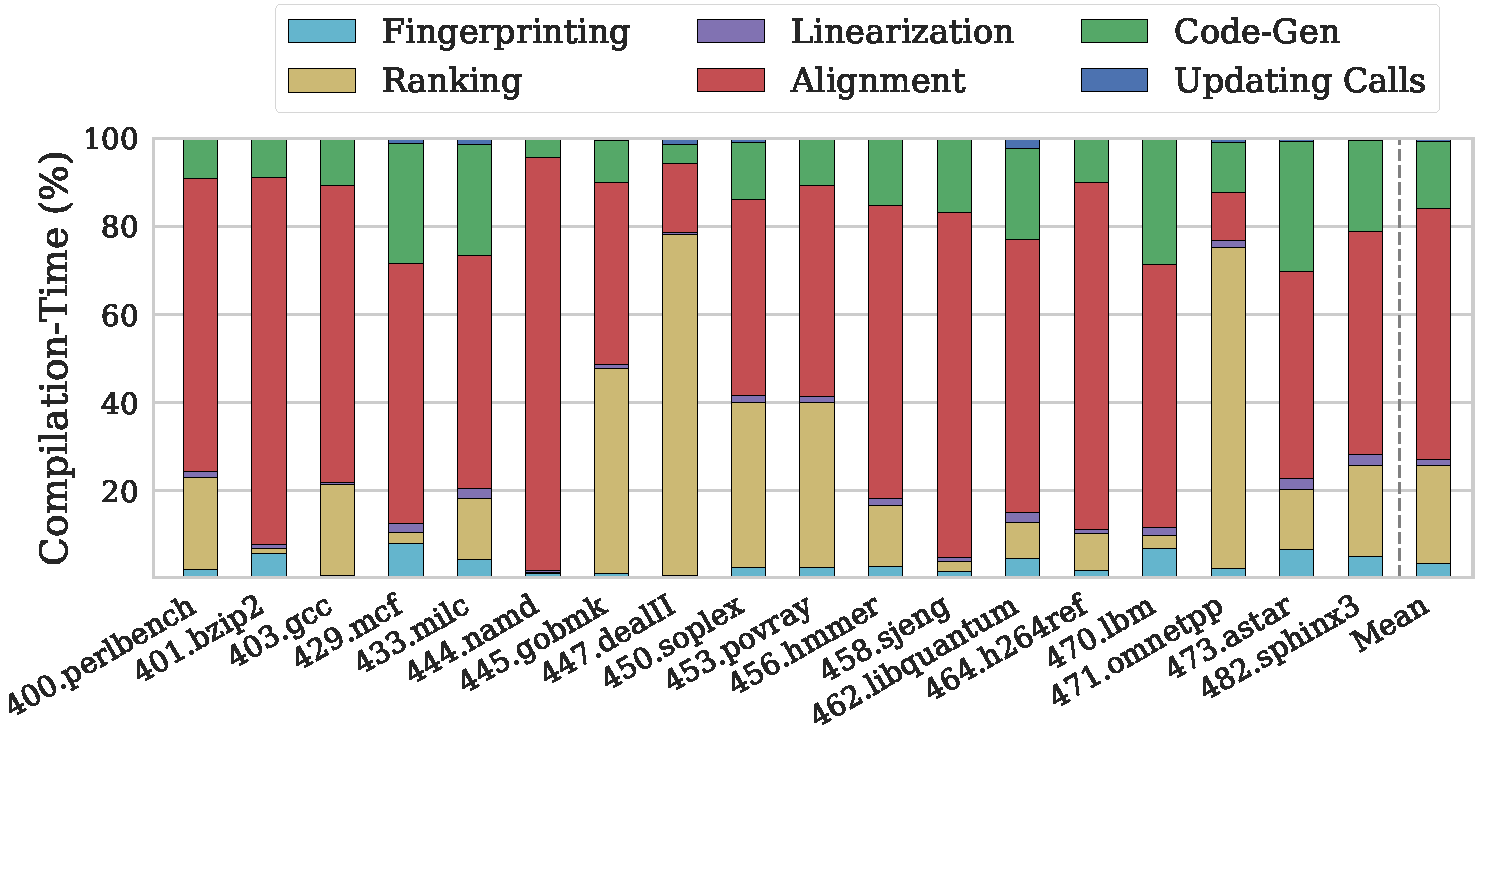
\includegraphics[width=1.0\linewidth]{figs/compilation-time-breakdown-sqrd.pdf}
  \vspace{-8.5ex}
  \caption{A compilation-time breakdown isolating the percentage for each major
           step of the optimization (t=1).}%, with an exploration threshold of one.}
  \label{fig:compilation-time-breakdown}
\end{figure}

\begin{figure*}[t]
  \centering
  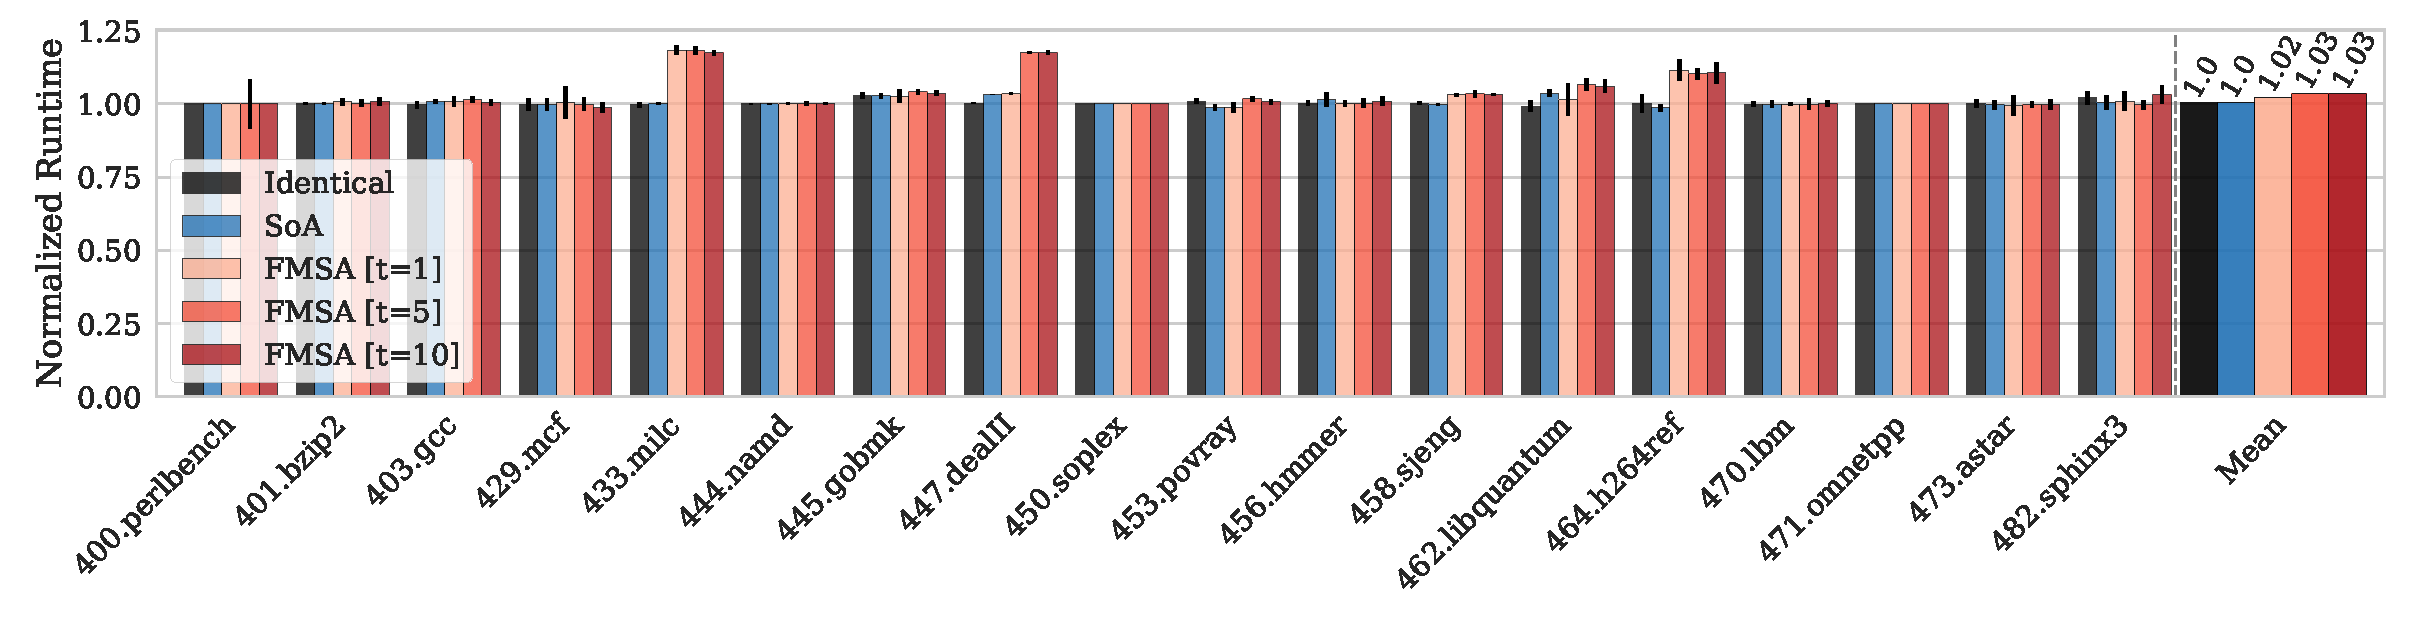
\includegraphics[width=\linewidth]{figs/runtime-impact.pdf}
  \vspace{-4ex}
  \caption{Runtime.}
  \label{fig:runtime-impact}
\end{figure*}

Unlike the other more mature implementations, our optimization is a prototype
implementation not yet highly tuned for compilation-time.
For this reason, we believe that the compilation-time overhead can be reduced
even further with enough egineering effort.
Nevertheless, the proposed ranking infrastructure is already able to reduce the
compilation-time overhead of the oracle by up to two orders of magnitude,
resulting in  an average compilation-time overhead of only 20\% compared to the
baseline, while still achieving a significant code-size reduction, very close to
the oracle.
We are able to close the gap between the ranking-based exploration and the
oracle at the cost of also increasing a compilation-time overhead.
However, note that the ranking-based exploration has a greedy strategy, while
the oracle selects the actual best candidate.
Therefore, even with an unlimited threshold, their results may still be slightly
different.

Figure~\ref{fig:compilation-time-breakdown} shows a detailed compilation-time
breakdown.
For each major step of the proposed optimization, we present the accumulated
time spent across the whole program.
In order to better understand the overhead of each one of the steps, we use
an exploration threshold of one ($t = 1$).
Because the ranking mechanism performs a quadratic operation on the number of
functions, computing the similarity between all pairs of functions, it is
expected that ranking would be amongst the most costly steps.
However, it is interesting to notice that the sequence alignment dominates most
of the compilation-time overhead, especially considering that this operation is
performed only once per function, when $t = 1$.
Although this operation is linear on the number of functions, the
Needleman-Wunsh algorithm~\cite{needleman70} is quadratic on the size of the
functions being aligned, both in time and space.
Unsurprisingly, the code generation is the third most costly step, which also
includes the time to optimize the merge of the parameters.
The remaining steps take, in total, a very small percentage of all the
compilation-time overhead.
This analysis suggests that optimizing the sequence alignment algorithm and
the ranking mechanism is key to reduce, even further, the overall
compilation-time overhead.

\vspace{-1ex}
\subsection{Performance Impact}


The primary goal of function merging is to reduce code size.
Nevertheless, it is also important to understand its impact on the programs'
execution time and the trade-offs between performance and code-size reduction.
Figure~\ref{fig:runtime-impact} shows the normalized execution time.
Overall, our optimization has an average impact of about 3\% on programs' performance.
For most of the programs, in the benchmark suite, there are no
statistical differences between the version optimized with the proposed function
merging or the baseline.
There are only a few benchmarks with a noticeable performance impact, namely,
433.milc, 447.dealII, and 464.h264ref.
%There are only three cases with a noticeable performance impact, namely,
%433.milc, 462.libquantum, and 464.h264ref.
%In particular, the 462.libquantum benchmark shows a performance degradation of
%about \todo{20\%}.

As a case study, we analyze the performance impact on the \text{433.milc}
benchmark.
We consider our function-merging optimization with exploration threshold equals
to one.
For this benchmark, a total of 58 functions were merged.
After inspecting the program's execution with profiling information, we
identified that only a handful of these functions are significantly hotter than
the other ones.
Hot basic blocks are determined based on the block frequencies recorded by
instrumenting all basic blocks in the program~\cite{ball94}.

If, instead, we prevent these hot function of being merged, the performance
impact goes away and we end up with a performance which is statistically
equivalent to the baseline version, while still providing a good code-size
reduction.
Our original optimization results in a code-size reduction of 5.11\% and a
performance overhead of about 18\%.
Even when reducing the performance overhead to zero, we can still offer a
code-size reduction of 2.09\%.
Note that the state-of-the-art has a reduction of only 1.09\% on this benchmark.
If we can be more permissive, allowing some of the hot functions to be merged,
we can have a code-size reduction of 3.43\% while keeping the performance impact
at about 8\%.

%However, \text{quantum\_gate1} is the largest function in the program,
%which means that this merge operation greatly contributes
%to the overall code-size reduction.
%Preventing this merge results in the code-size reduction dropping from 16\% to
%6.9\%, which is still a very significant code-size reduction compared to the
%other techniques that show no reduction on this particular benchmark.

%It is interesting to note that, for the 447.dealII benchmark, FMSA [t=1] has
%no extra impact than the state-of-the-art


%As a case study, we analyze the performance impact on the \text{462.libquantum}
%benchmark.
%After a detailed inspection of the program's execution with profiling
%information, we identified only two functions that contain the hottest basic
%blocks in the whole program.
%Hot basic blocks are determined based on the block frequencies recorded by
%instrumenting all basic blocks in the program~\cite{ball94}.
%The two hottest functions are: \text{quantum\_gate1} and
%\text{quantum\_decohere}.
%If we cross this information with the list of merged functions, we can confirm
%that the function \text{quantum\_gate1} is involved in a merge operation with
%a non-identical function.

%If, instead, we prevent this function of being merged, the performance
%impact goes away and we end up with a performance which is statistically
%equivalent to the baseline version.
%However, \text{quantum\_gate1} is the largest function in the program,
%which means that this merge operation greatly contributes
%to the overall code-size reduction.
%Preventing this merge results in the code-size reduction dropping from 16\% to
%6.9\%, which is still a very significant code-size reduction compared to the
%other techniques that show no reduction on this particular benchmark.
